\section{Additional results for Experiment 1}
\label{app:exp1}

All intervals in this appendix are 95\% history-bootstrap intervals (Section~\ref{sec:inference}).

\subsection{Query relevance by construction and order}

Table~\ref{tab:main} and Figure~\ref{fig:construction-order} give $R$ for every construction and order group, and Table~\ref{tab:frozen} the three superseded-minus-control contrasts that tested the original hypothesis. Superseded and other-attribute relevance are positive and similar in both order groups; entity-mention relevance is the largest among the non-live constructions; unassigned relevance is near zero overall but large and of opposite sign in the two order groups.

\begin{table}[t]
\caption{Query relevance $R$ (nats) by construction and order group in Experiment 1, with 95\% history-bootstrap intervals over 96 histories. The live control has one assignment block, so it has no order split.}
\label{tab:main}
\begin{center}
\small
\begin{tabular}{@{}llrrr@{}}
\toprule
Model & Construction & Overall $R$ & Aligned $R$ & Reversed $R$ \\
\midrule
Qwen3-8B & Live & 32.598 [31.258, 33.967] & — & — \\
Qwen3-8B & Superseded & 1.974 [1.840, 2.109] & 2.144 [1.995, 2.301] & 1.804 [1.660, 1.947] \\
Qwen3-8B & Other attribute & 1.660 [1.488, 1.835] & 1.679 [1.527, 1.835] & 1.641 [1.422, 1.863] \\
Qwen3-8B & Entity mention & 5.478 [5.128, 5.825] & 4.493 [4.235, 4.770] & 6.463 [5.971, 6.940] \\
Qwen3-8B & Early unassigned & −0.037 [−0.203, 0.121] & 3.252 [3.046, 3.455] & −3.327 [−3.518, −3.150] \\
Qwen3-8B & Late unassigned & 0.001 [−0.208, 0.211] & 3.187 [2.948, 3.442] & −3.184 [−3.433, −2.945] \\
\midrule
Gemma 3 4B & Live & 39.355 [38.303, 40.415] & — & — \\
Gemma 3 4B & Superseded & 1.688 [1.568, 1.817] & 1.703 [1.574, 1.841] & 1.672 [1.529, 1.831] \\
Gemma 3 4B & Other attribute & 1.683 [1.541, 1.832] & 1.763 [1.598, 1.932] & 1.603 [1.453, 1.771] \\
Gemma 3 4B & Entity mention & 4.277 [4.029, 4.545] & 5.181 [4.884, 5.496] & 3.372 [3.131, 3.633] \\
Gemma 3 4B & Early unassigned & 0.113 [−0.023, 0.245] & 2.598 [2.395, 2.798] & −2.372 [−2.567, −2.178] \\
Gemma 3 4B & Late unassigned & 0.125 [−0.055, 0.305] & 3.445 [3.202, 3.696] & −3.194 [−3.447, −2.945] \\
\bottomrule
\end{tabular}
\end{center}
\end{table}

\begin{figure}[t]
\begin{center}
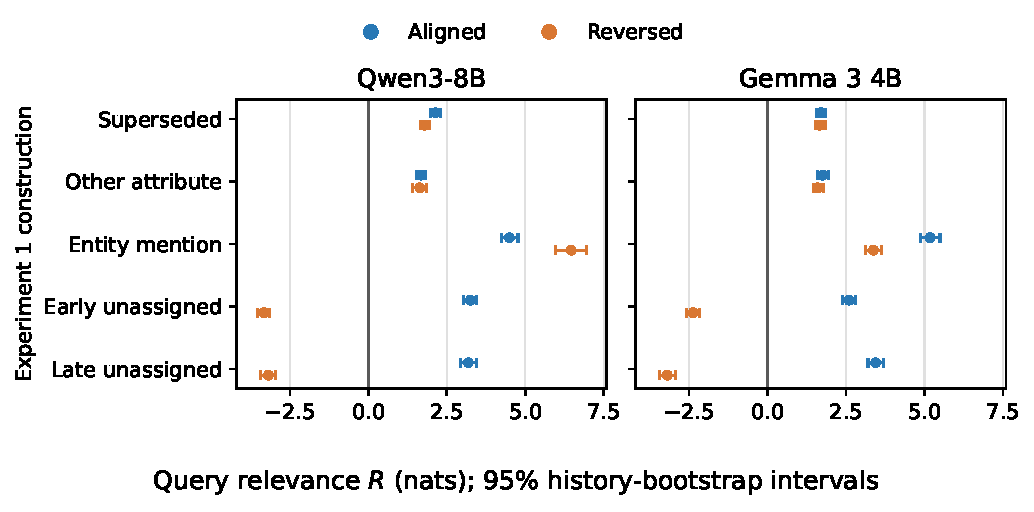
\includegraphics[width=0.98\linewidth]{figures/construction_by_order.pdf}
\end{center}
\caption{Query relevance $R$ (nats) for the five non-live constructions of Experiment 1, by order group and model. Points are means over 96 histories; intervals are 95\% history-bootstrap intervals. Live is omitted from the shared scale (Table~\ref{tab:main}). Paired order differences are in Table~\ref{tab:b-paired-r}.}
\label{fig:construction-order}
\end{figure}

\begin{table}[t]
\caption{Superseded minus each control construction, $R_{\text{superseded}}-R_{\text{control}}$ (nats), with 95\% history-bootstrap intervals over 96 histories. Because early-unassigned $R$ is near zero after averaging over orders (Section~\ref{sec:order}), the last contrast is close to superseded $R$ itself. Order-stratified versions are in Table~\ref{tab:b-order}.}
\label{tab:frozen}
\begin{center}
\small
\begin{tabular}{@{}llrr@{}}
\toprule
Control & Isolates & Qwen3-8B & Gemma 3 4B \\
\midrule
Other attribute & relation status & 0.314 [0.147, 0.482] & 0.004 [−0.104, 0.118] \\
Entity mention & construction & −3.504 [−3.806, −3.198] & −2.589 [−2.829, −2.361] \\
Early unassigned & none: order-averaged control near zero & 2.011 [1.855, 2.170] & 1.575 [1.440, 1.719] \\
\bottomrule
\end{tabular}
\end{center}
\end{table}

\subsection{Order groups}

Table~\ref{tab:b-paired-r} gives the paired order effect on $R$ itself for each construction, Table~\ref{tab:b-order} each superseded-minus-control contrast by order group, and Table~\ref{tab:b-paired} the paired difference between the aligned and reversed contrasts. Paired differences are computed within history. The live control has one assignment block and no order split.

\begin{figure}[h]
\begin{center}
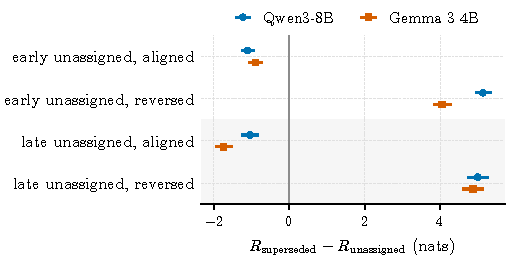
\includegraphics[width=0.58\linewidth]{figures/order_stratified_contrasts.pdf}
\end{center}
\caption{Superseded-minus-unassigned relevance contrasts by order group, in nats, with 95\% history-bootstrap intervals. The contrasts are negative under aligned order and positive under reversed order in both models. The comparison depends on both construction and order; it does not imply that construction is irrelevant.}
\label{fig:order}
\end{figure}

\begin{table}[h]
\caption{Paired order effect on query relevance, $R_{\text{aligned}}-R_{\text{reversed}}$ (nats), computed within history, with the fraction of the 96 histories in which it is positive.}
\label{tab:b-paired-r}
\begin{center}
\small
\begin{tabular}{@{}lrr@{}}
\toprule
Construction & Qwen3-8B & Gemma 3 4B \\
\midrule
Superseded & 0.340 [0.218, 0.470]; 0.688 & 0.032 [−0.101, 0.168]; 0.531 \\
Entity mention & −1.969 [−2.344, −1.604]; 0.135 & 1.810 [1.580, 2.058]; 0.958 \\
Early unassigned & 6.578 [6.356, 6.789]; 1.000 & 4.970 [4.700, 5.257]; 1.000 \\
Late unassigned & 6.371 [6.113, 6.646]; 1.000 & 6.639 [6.308, 6.967]; 1.000 \\
\bottomrule
\end{tabular}
\end{center}
\end{table}

\begin{table}[h]
\caption{Superseded minus control, $R_{\text{superseded}}-R_{\text{control}}$ (nats), by order group. Overall values are in Table~\ref{tab:frozen}.}
\label{tab:b-order}
\begin{center}
\small
\begin{tabular}{@{}llrr@{}}
\toprule
Control & Order & Qwen3-8B & Gemma 3 4B \\
\midrule
Other attribute & Aligned & 0.465 [0.295, 0.649] & −0.060 [−0.215, 0.099] \\
Other attribute & Reversed & 0.162 [−0.049, 0.367] & 0.069 [−0.080, 0.213] \\
Entity mention & Aligned & −2.350 [−2.572, −2.125] & −3.478 [−3.769, −3.197] \\
Entity mention & Reversed & −4.659 [−5.119, −4.207] & −1.700 [−1.946, −1.465] \\
Early unassigned & Aligned & −1.108 [−1.281, −0.925] & −0.895 [−1.084, −0.719] \\
Early unassigned & Reversed & 5.130 [4.920, 5.348] & 4.044 [3.810, 4.292] \\
Late unassigned & Overall & 1.973 [1.762, 2.183] & 1.562 [1.390, 1.742] \\
Late unassigned & Aligned & −1.043 [−1.281, −0.810] & −1.741 [−1.968, −1.505] \\
Late unassigned & Reversed & 4.988 [4.724, 5.266] & 4.866 [4.592, 5.155] \\
\bottomrule
\end{tabular}
\end{center}
\end{table}

\begin{table}[h]
\caption{Paired aligned-minus-reversed differences in the superseded-minus-control contrast (nats).}
\label{tab:b-paired}
\begin{center}
\small
\begin{tabular}{@{}lrr@{}}
\toprule
Control & Qwen3-8B & Gemma 3 4B \\
\midrule
Other attribute & 0.302 [0.103, 0.509] & −0.128 [−0.323, 0.081] \\
Entity mention & 2.309 [1.933, 2.707] & −1.778 [−2.049, −1.519] \\
Early unassigned & −6.238 [−6.481, −5.983] & −4.939 [−5.275, −4.620] \\
Late unassigned & −6.031 [−6.307, −5.754] & −6.607 [−6.951, −6.243] \\
\bottomrule
\end{tabular}
\end{center}
\end{table}

\subsection{Accuracy and correctly answered histories}

Table~\ref{tab:b-accuracy} gives strict rank-one accuracy over all 3,072 scored prompts per construction in the main experiment, counting baseline and edited prompts and repeated renderings of identical prompts.

\begin{table}[h]
\caption{Strict rank-one candidate accuracy in Experiment 1, per construction.}
\label{tab:b-accuracy}
\begin{center}
\small
\begin{tabular}{@{}lrr@{}}
\toprule
Construction & Qwen3-8B & Gemma 3 4B \\
\midrule
Live & 3,064/3,072 (99.7396\%) & 3,072/3,072 (100\%) \\
Superseded & 3,072/3,072 (100\%) & 3,072/3,072 (100\%) \\
Other attribute & 3,072/3,072 (100\%) & 3,072/3,072 (100\%) \\
Entity mention & 3,072/3,072 (100\%) & 3,072/3,072 (100\%) \\
Early unassigned & 3,072/3,072 (100\%) & 3,071/3,072 (99.9674\%) \\
Late unassigned & 3,069/3,072 (99.9023\%) & 3,072/3,072 (100\%) \\
\bottomrule
\end{tabular}
\end{center}
\end{table}

Restricting the analysis to histories in which every prompt was answered correctly retains 91/96 Qwen and 95/96 Gemma histories and leaves the contrasts essentially unchanged (Table~\ref{tab:b-selected}).

\begin{table}[h]
\caption{Superseded minus control (nats) among histories with every prompt ranked correctly.}
\label{tab:b-selected}
\begin{center}
\small
\begin{tabular}{@{}lrr@{}}
\toprule
Control & Qwen3-8B (91 histories) & Gemma 3 4B (95 histories) \\
\midrule
Other attribute & 0.371 [0.201, 0.532] & 0.004 [−0.106, 0.119] \\
Entity mention & −3.445 [−3.750, −3.141] & −2.591 [−2.827, −2.354] \\
Early unassigned & 2.015 [1.861, 2.176] & 1.576 [1.433, 1.714] \\
\bottomrule
\end{tabular}
\end{center}
\end{table}

\subsection{Source and donor score changes}
\label{app:score-changes}

Table~\ref{tab:b-abs-mass} gives the absolute log masses of the source, donor, and current candidates before and after the edit, and Table~\ref{tab:b-score-changes} the mean changes. The source and donor masses are low in every construction except live, so a change of several nats between them does not imply that probability moves from one to the other.

\begin{table}[h]
\caption{Absolute candidate log masses $S$ (nats) in Experiment 1: mean over prompts, with the first and third quartiles below. Source is the edited earlier value, donor its replacement, current the correct answer; 1,536 baseline and 1,536 edited prompts per construction and model. In the live construction the source is the current value of the edited entity, so its mass is high when that entity is queried.}
\label{tab:b-abs-mass}
\begin{center}
\resizebox{\linewidth}{!}{%
\begin{tabular}{@{}lrrrrrr@{}}
\toprule
 & \multicolumn{2}{c}{Source} & \multicolumn{2}{c}{Donor} & \multicolumn{2}{c}{Current} \\
\cmidrule(lr){2-3}\cmidrule(lr){4-5}\cmidrule(l){6-7}
Construction & Baseline & Edited & Baseline & Edited & Baseline & Edited \\
\midrule
\multicolumn{7}{@{}l}{\emph{Qwen3-8B}} \\
Live & \shortstack[r]{−8.027\\[-1pt]\scriptsize(−16.124, −0.000)} & \shortstack[r]{−23.650\\[-1pt]\scriptsize(−26.373, −20.584)} & \shortstack[r]{−24.086\\[-1pt]\scriptsize(−26.850, −20.941)} & \shortstack[r]{−8.132\\[-1pt]\scriptsize(−16.394, −0.000)} & \shortstack[r]{−0.004\\[-1pt]\scriptsize(−0.000, −0.000)} & \shortstack[r]{−0.012\\[-1pt]\scriptsize(−0.000, −0.000)} \\
Superseded & \shortstack[r]{−22.271\\[-1pt]\scriptsize(−24.703, −19.578)} & \shortstack[r]{−23.881\\[-1pt]\scriptsize(−26.425, −21.172)} & \shortstack[r]{−23.618\\[-1pt]\scriptsize(−25.922, −20.888)} & \shortstack[r]{−22.120\\[-1pt]\scriptsize(−24.476, −19.328)} & \shortstack[r]{−0.000\\[-1pt]\scriptsize(−0.000, −0.000)} & \shortstack[r]{−0.000\\[-1pt]\scriptsize(−0.000, −0.000)} \\
Other attribute & \shortstack[r]{−21.048\\[-1pt]\scriptsize(−23.317, −18.476)} & \shortstack[r]{−22.396\\[-1pt]\scriptsize(−24.662, −19.810)} & \shortstack[r]{−22.234\\[-1pt]\scriptsize(−24.235, −19.717)} & \shortstack[r]{−20.903\\[-1pt]\scriptsize(−22.978, −18.297)} & \shortstack[r]{−0.000\\[-1pt]\scriptsize(−0.000, −0.000)} & \shortstack[r]{−0.000\\[-1pt]\scriptsize(−0.000, −0.000)} \\
Entity mention & \shortstack[r]{−19.836\\[-1pt]\scriptsize(−23.242, −16.699)} & \shortstack[r]{−23.668\\[-1pt]\scriptsize(−26.370, −20.562)} & \shortstack[r]{−23.452\\[-1pt]\scriptsize(−26.000, −20.390)} & \shortstack[r]{−19.868\\[-1pt]\scriptsize(−23.344, −16.464)} & \shortstack[r]{−0.001\\[-1pt]\scriptsize(−0.000, −0.000)} & \shortstack[r]{−0.001\\[-1pt]\scriptsize(−0.000, −0.000)} \\
Early unassigned & \shortstack[r]{−16.488\\[-1pt]\scriptsize(−18.781, −14.193)} & \shortstack[r]{−20.697\\[-1pt]\scriptsize(−22.808, −18.257)} & \shortstack[r]{−20.497\\[-1pt]\scriptsize(−22.524, −18.016)} & \shortstack[r]{−16.485\\[-1pt]\scriptsize(−18.609, −13.922)} & \shortstack[r]{−0.000\\[-1pt]\scriptsize(−0.000, −0.000)} & \shortstack[r]{−0.000\\[-1pt]\scriptsize(−0.000, −0.000)} \\
Late unassigned & \shortstack[r]{−17.218\\[-1pt]\scriptsize(−19.385, −14.906)} & \shortstack[r]{−23.119\\[-1pt]\scriptsize(−25.287, −20.589)} & \shortstack[r]{−22.899\\[-1pt]\scriptsize(−25.107, −20.467)} & \shortstack[r]{−17.216\\[-1pt]\scriptsize(−19.365, −15.031)} & \shortstack[r]{−0.004\\[-1pt]\scriptsize(−0.000, −0.000)} & \shortstack[r]{−0.004\\[-1pt]\scriptsize(−0.000, −0.000)} \\
\multicolumn{7}{@{}l}{\emph{Gemma 3 4B}} \\
Live & \shortstack[r]{−9.784\\[-1pt]\scriptsize(−19.619, −0.000)} & \shortstack[r]{−24.049\\[-1pt]\scriptsize(−26.585, −21.125)} & \shortstack[r]{−24.191\\[-1pt]\scriptsize(−27.076, −20.906)} & \shortstack[r]{−10.049\\[-1pt]\scriptsize(−20.275, −0.000)} & \shortstack[r]{−0.000\\[-1pt]\scriptsize(−0.000, −0.000)} & \shortstack[r]{−0.000\\[-1pt]\scriptsize(−0.000, −0.000)} \\
Superseded & \shortstack[r]{−24.311\\[-1pt]\scriptsize(−26.603, −22.109)} & \shortstack[r]{−25.552\\[-1pt]\scriptsize(−27.981, −23.386)} & \shortstack[r]{−25.498\\[-1pt]\scriptsize(−27.876, −23.237)} & \shortstack[r]{−24.268\\[-1pt]\scriptsize(−26.601, −21.979)} & \shortstack[r]{−0.000\\[-1pt]\scriptsize(−0.000, −0.000)} & \shortstack[r]{−0.000\\[-1pt]\scriptsize(−0.000, −0.000)} \\
Other attribute & \shortstack[r]{−23.486\\[-1pt]\scriptsize(−25.900, −21.062)} & \shortstack[r]{−24.929\\[-1pt]\scriptsize(−27.427, −22.533)} & \shortstack[r]{−24.734\\[-1pt]\scriptsize(−27.127, −22.564)} & \shortstack[r]{−23.621\\[-1pt]\scriptsize(−25.952, −21.291)} & \shortstack[r]{−0.000\\[-1pt]\scriptsize(−0.000, −0.000)} & \shortstack[r]{−0.001\\[-1pt]\scriptsize(−0.000, −0.000)} \\
Entity mention & \shortstack[r]{−20.540\\[-1pt]\scriptsize(−23.446, −17.851)} & \shortstack[r]{−23.749\\[-1pt]\scriptsize(−26.189, −21.445)} & \shortstack[r]{−23.606\\[-1pt]\scriptsize(−25.977, −21.137)} & \shortstack[r]{−20.650\\[-1pt]\scriptsize(−23.591, −17.786)} & \shortstack[r]{−0.000\\[-1pt]\scriptsize(−0.000, −0.000)} & \shortstack[r]{−0.000\\[-1pt]\scriptsize(−0.000, −0.000)} \\
Early unassigned & \shortstack[r]{−20.919\\[-1pt]\scriptsize(−23.138, −18.691)} & \shortstack[r]{−24.235\\[-1pt]\scriptsize(−26.460, −22.135)} & \shortstack[r]{−23.971\\[-1pt]\scriptsize(−26.234, −21.627)} & \shortstack[r]{−20.996\\[-1pt]\scriptsize(−23.279, −18.750)} & \shortstack[r]{−0.000\\[-1pt]\scriptsize(−0.000, −0.000)} & \shortstack[r]{−0.004\\[-1pt]\scriptsize(−0.000, −0.000)} \\
Late unassigned & \shortstack[r]{−20.887\\[-1pt]\scriptsize(−23.310, −18.196)} & \shortstack[r]{−25.398\\[-1pt]\scriptsize(−28.104, −22.651)} & \shortstack[r]{−25.138\\[-1pt]\scriptsize(−27.712, −22.286)} & \shortstack[r]{−21.139\\[-1pt]\scriptsize(−23.869, −18.339)} & \shortstack[r]{−0.000\\[-1pt]\scriptsize(−0.000, −0.000)} & \shortstack[r]{−0.000\\[-1pt]\scriptsize(−0.000, −0.000)} \\
\bottomrule
\end{tabular}}
\end{center}
\end{table}

Table~\ref{tab:b-score-changes} gives the mean baseline-to-edit change in the source and donor scores, averaged over both queries; their difference is the mean edit effect $E$. Unlike $R$, $E$ does not subtract the other query's effect. These are means over prompt pairs without intervals. Because the scores are log masses, exponentiating a mean gives a geometric mean of masses. The current answer's mean log mass rounds to 0.000 before and after editing in every non-live construction except Qwen's late unassigned (−0.004) and entity mention (−0.001) and Gemma's early unassigned (−0.004 after editing) and other attribute (−0.001 after editing).

\begin{table}[h]
\caption{Mean source and donor log-mass changes and mean edit effect $E$ (nats).}
\label{tab:b-score-changes}
\begin{center}
\small
\begin{tabular}{@{}llrrr@{}}
\toprule
Model & Construction & Source change & Donor change & Mean $E$ \\
\midrule
Qwen3-8B & Superseded & −1.610 & 1.497 & 3.108 \\
Qwen3-8B & Other attribute & −1.348 & 1.331 & 2.679 \\
Qwen3-8B & Entity mention & −3.832 & 3.584 & 7.417 \\
Qwen3-8B & Early unassigned & −4.208 & 4.012 & 8.221 \\
Qwen3-8B & Late unassigned & −5.901 & 5.682 & 11.583 \\
\midrule
Gemma 3 4B & Superseded & −1.241 & 1.230 & 2.471 \\
Gemma 3 4B & Other attribute & −1.444 & 1.113 & 2.557 \\
Gemma 3 4B & Entity mention & −3.209 & 2.957 & 6.166 \\
Gemma 3 4B & Early unassigned & −3.315 & 2.975 & 6.290 \\
Gemma 3 4B & Late unassigned & −4.511 & 3.999 & 8.510 \\
\bottomrule
\end{tabular}
\end{center}
\end{table}

\subsection{Target attributes}

Each target attribute contributes 24 histories. Superseded minus entity mention is negative for every attribute in both models (Table~\ref{tab:b-attr-entity}); superseded minus other attribute varies by attribute in Qwen and has intervals spanning zero for every attribute in Gemma (Table~\ref{tab:b-attr-other}).

\begin{table}[h]
\caption{Superseded minus entity mention by target attribute (nats; 24 histories each).}
\label{tab:b-attr-entity}
\begin{center}
\small
\begin{tabular}{@{}lrr@{}}
\toprule
Attribute & Qwen3-8B & Gemma 3 4B \\
\midrule
Badge & −4.310 [−4.819, −3.787] & −1.794 [−2.047, −1.556] \\
Color & −1.794 [−2.129, −1.469] & −2.532 [−2.852, −2.203] \\
Code & −4.570 [−5.098, −4.058] & −3.937 [−4.418, −3.452] \\
Label & −3.342 [−3.668, −3.017] & −2.094 [−2.358, −1.809] \\
\bottomrule
\end{tabular}
\end{center}
\end{table}

\begin{table}[h]
\caption{Superseded minus other attribute by target attribute (nats; 24 histories each).}
\label{tab:b-attr-other}
\begin{center}
\small
\begin{tabular}{@{}lrr@{}}
\toprule
Attribute & Qwen3-8B & Gemma 3 4B \\
\midrule
Badge & 0.748 [0.512, 0.969] & 0.011 [−0.206, 0.232] \\
Color & 0.876 [0.683, 1.068] & −0.028 [−0.236, 0.208] \\
Code & −0.570 [−0.866, −0.280] & −0.045 [−0.292, 0.217] \\
Label & 0.200 [−0.042, 0.459] & 0.078 [−0.110, 0.264] \\
\bottomrule
\end{tabular}
\end{center}
\end{table}

\subsection{Cell-stratified bootstrap}

The primary bootstrap resamples histories without regard to the 48 entity-pair $\times$ attribute $\times$ name-assignment cells. As a sensitivity check we resampled two histories with replacement within each cell on every draw (2,000 draws), which holds the cell counts fixed. Means are unchanged, intervals narrow, and every conclusion about the sign of a contrast is preserved (Table~\ref{tab:b-stratified}).

\begin{table}[h]
\caption{Superseded minus control (nats) with cell-stratified bootstrap intervals.}
\label{tab:b-stratified}
\begin{center}
\small
\begin{tabular}{@{}lrr@{}}
\toprule
Control & Qwen3-8B & Gemma 3 4B \\
\midrule
Other attribute & 0.314 [0.225, 0.403] & 0.004 [−0.079, 0.090] \\
Entity mention & −3.504 [−3.641, −3.363] & −2.589 [−2.707, −2.475] \\
Early unassigned & 2.011 [1.920, 2.100] & 1.575 [1.477, 1.667] \\
\bottomrule
\end{tabular}
\end{center}
\end{table}

\FloatBarrier
